\subsection{Combine cut-based Analysis 7 TeV and 8 TeV OF}


%%%%%%%%%%%%%%%%%%%%%%%%%%%%%%
\begin{figure}[!hbtp]
\centering
\subfigure[SM Higgs (cut-based) 7 TeV 0/1/2-Jets ]{
\centering
\label{subfig:sm_cut_7tev}
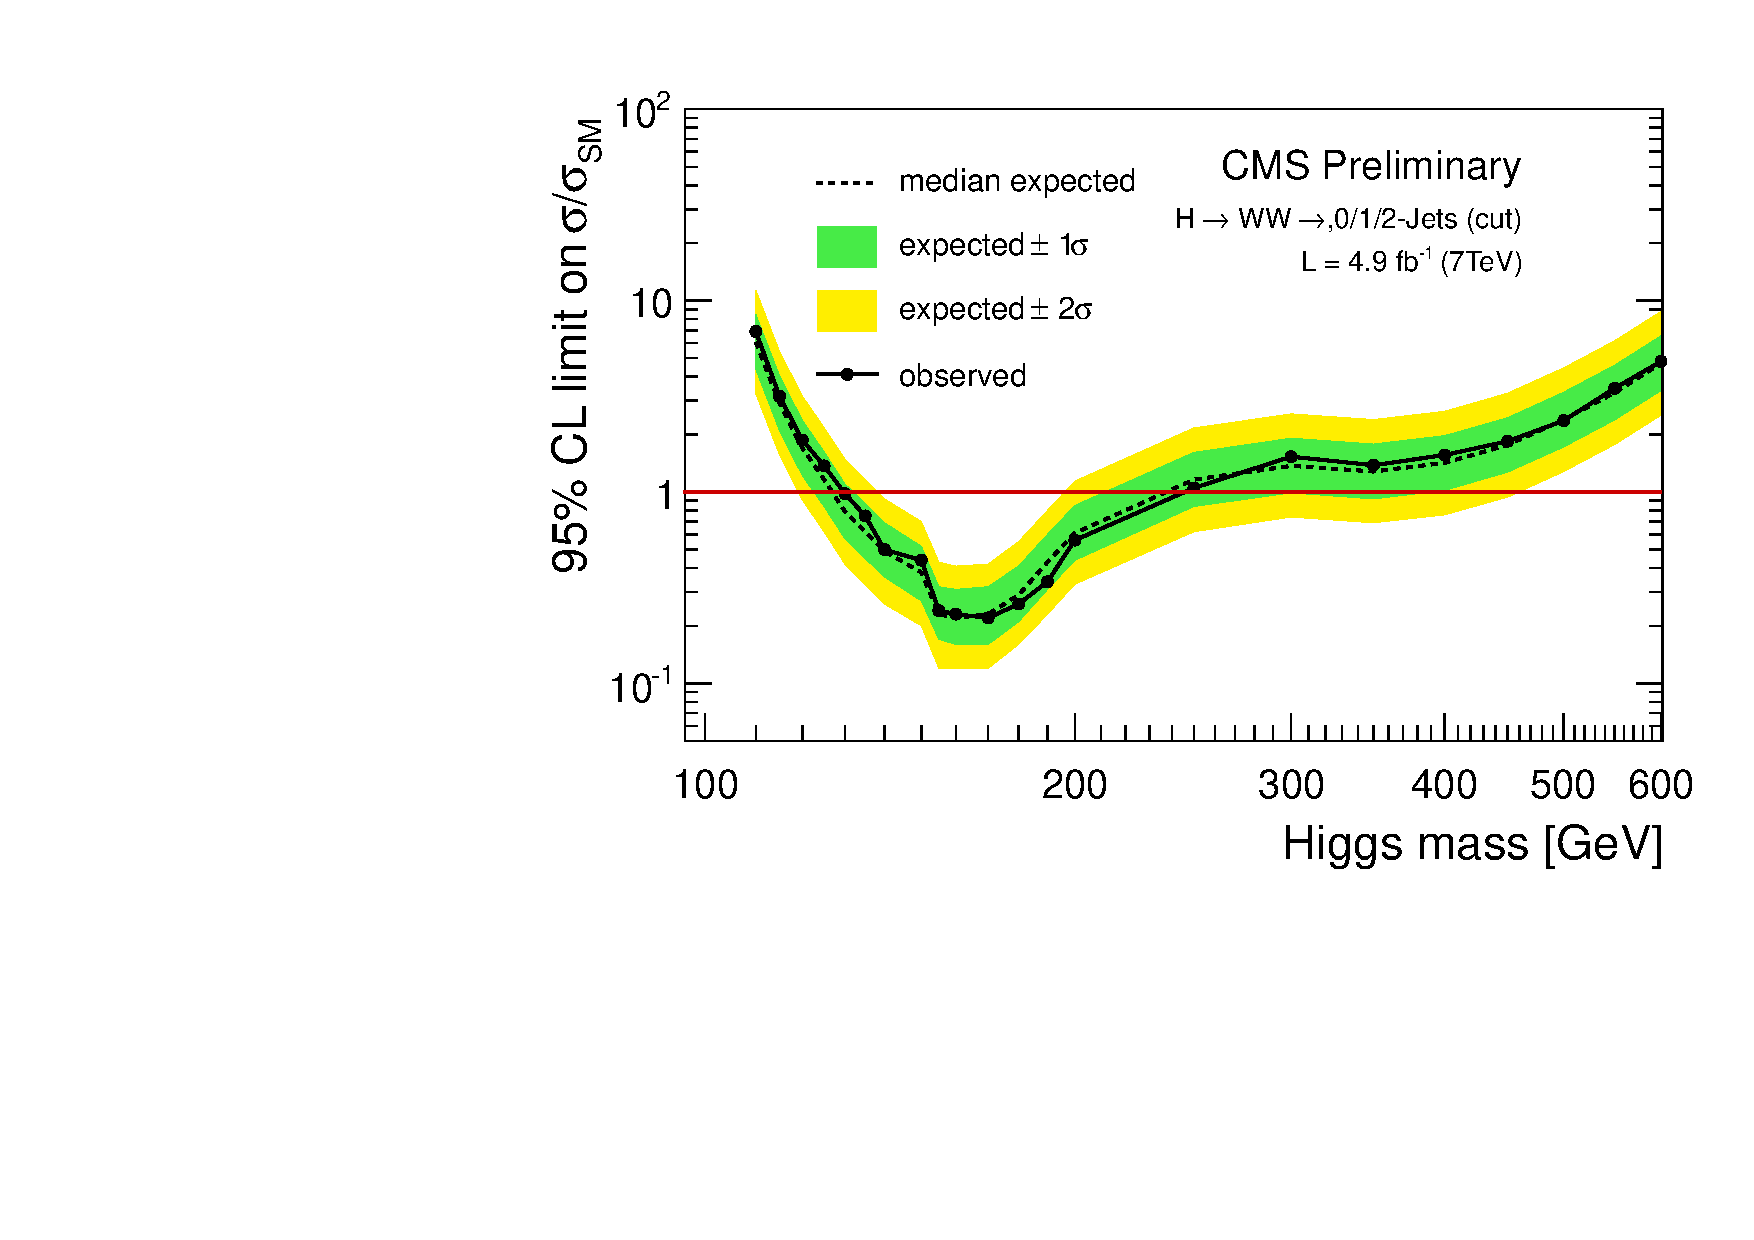
\includegraphics[width=.45\textwidth]{figures/limits_nj_cut_7TeV-CLs-asymptotic_log.pdf}}
\centering
\subfigure[SM Higgs (cut-based) 8 TeV 0/1-Jet OF ]{
\centering
\label{subfig:sm_cut_8tev}
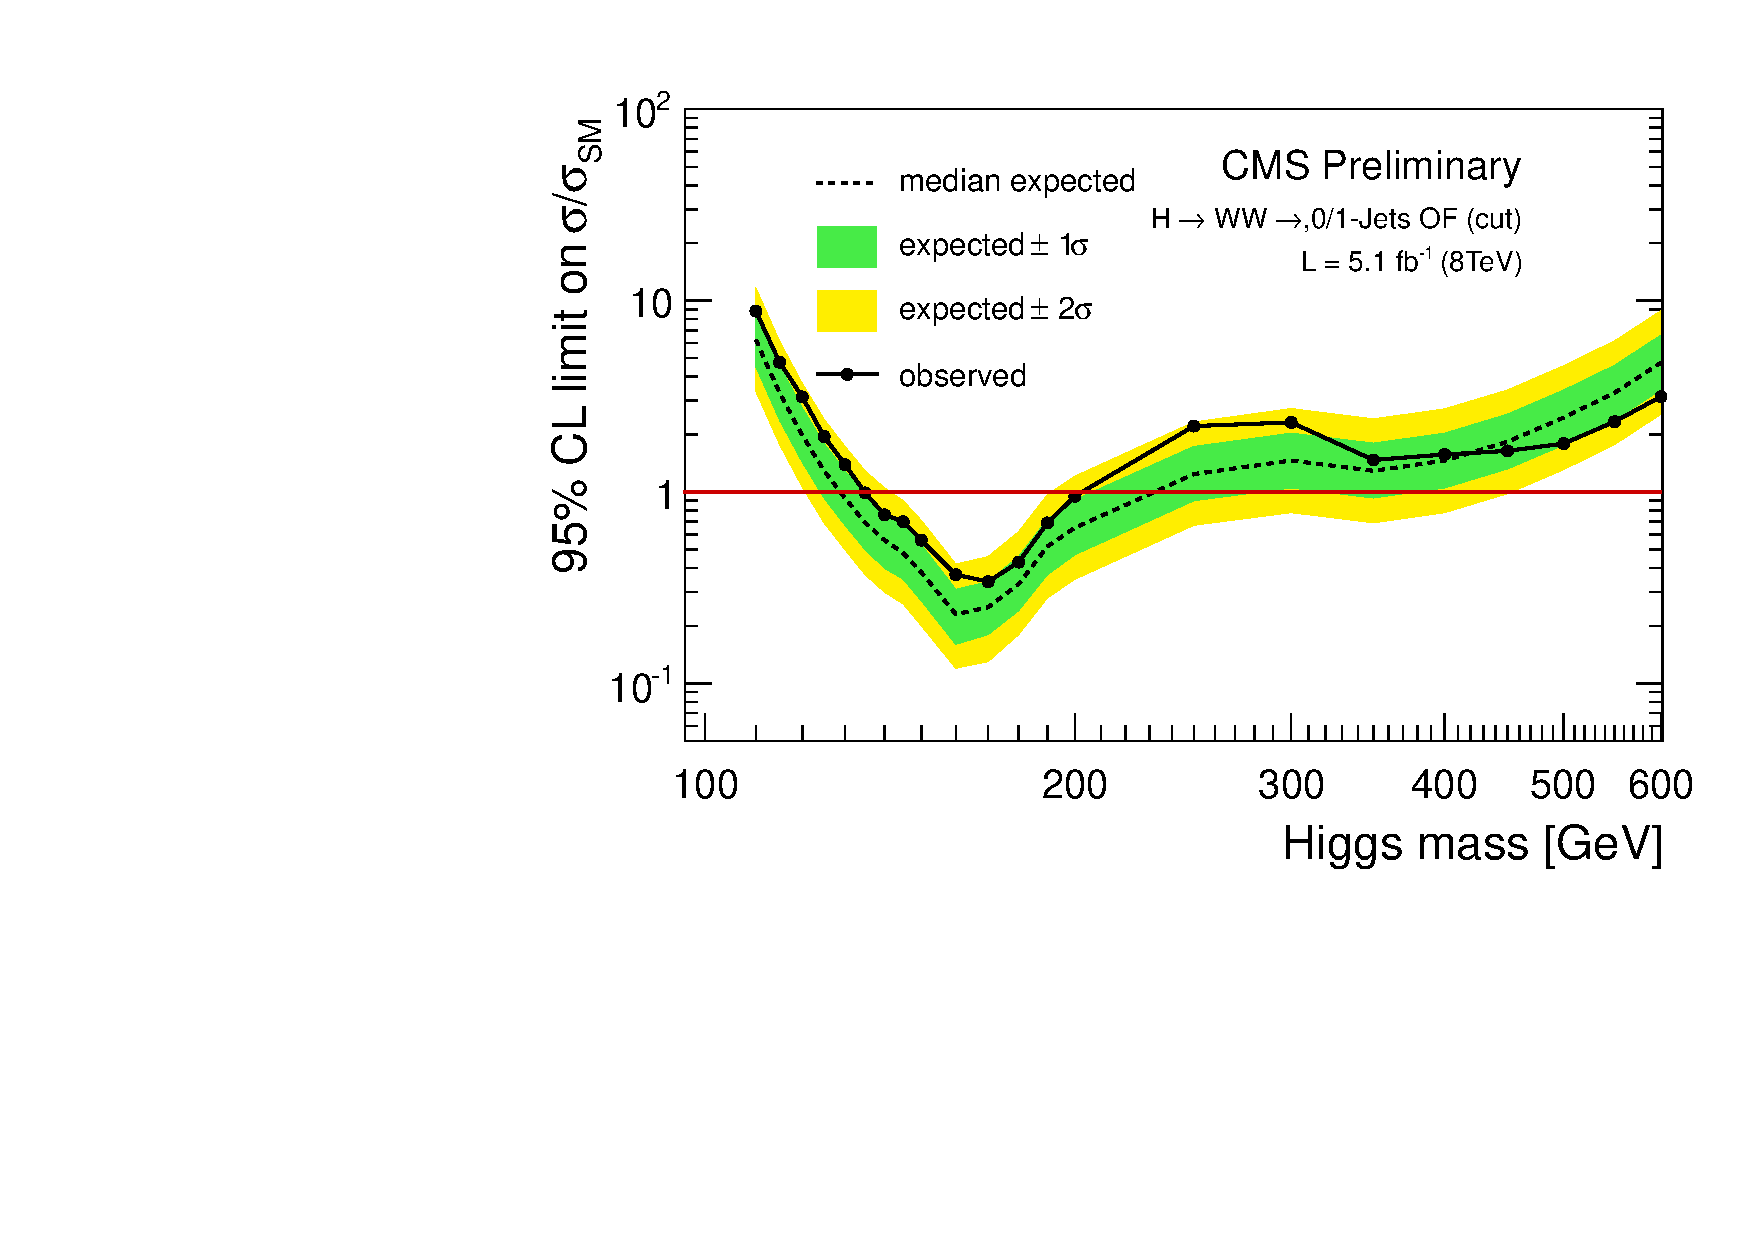
\includegraphics[width=.45\textwidth]{figures/limits_njof_cut_8TeV-CLs-asymptotic_log.pdf}} \\
\subfigure[SM Higgs (cut-based) 7+8 TeV ]{
\centering
\label{subfig:sm_cut_comb}
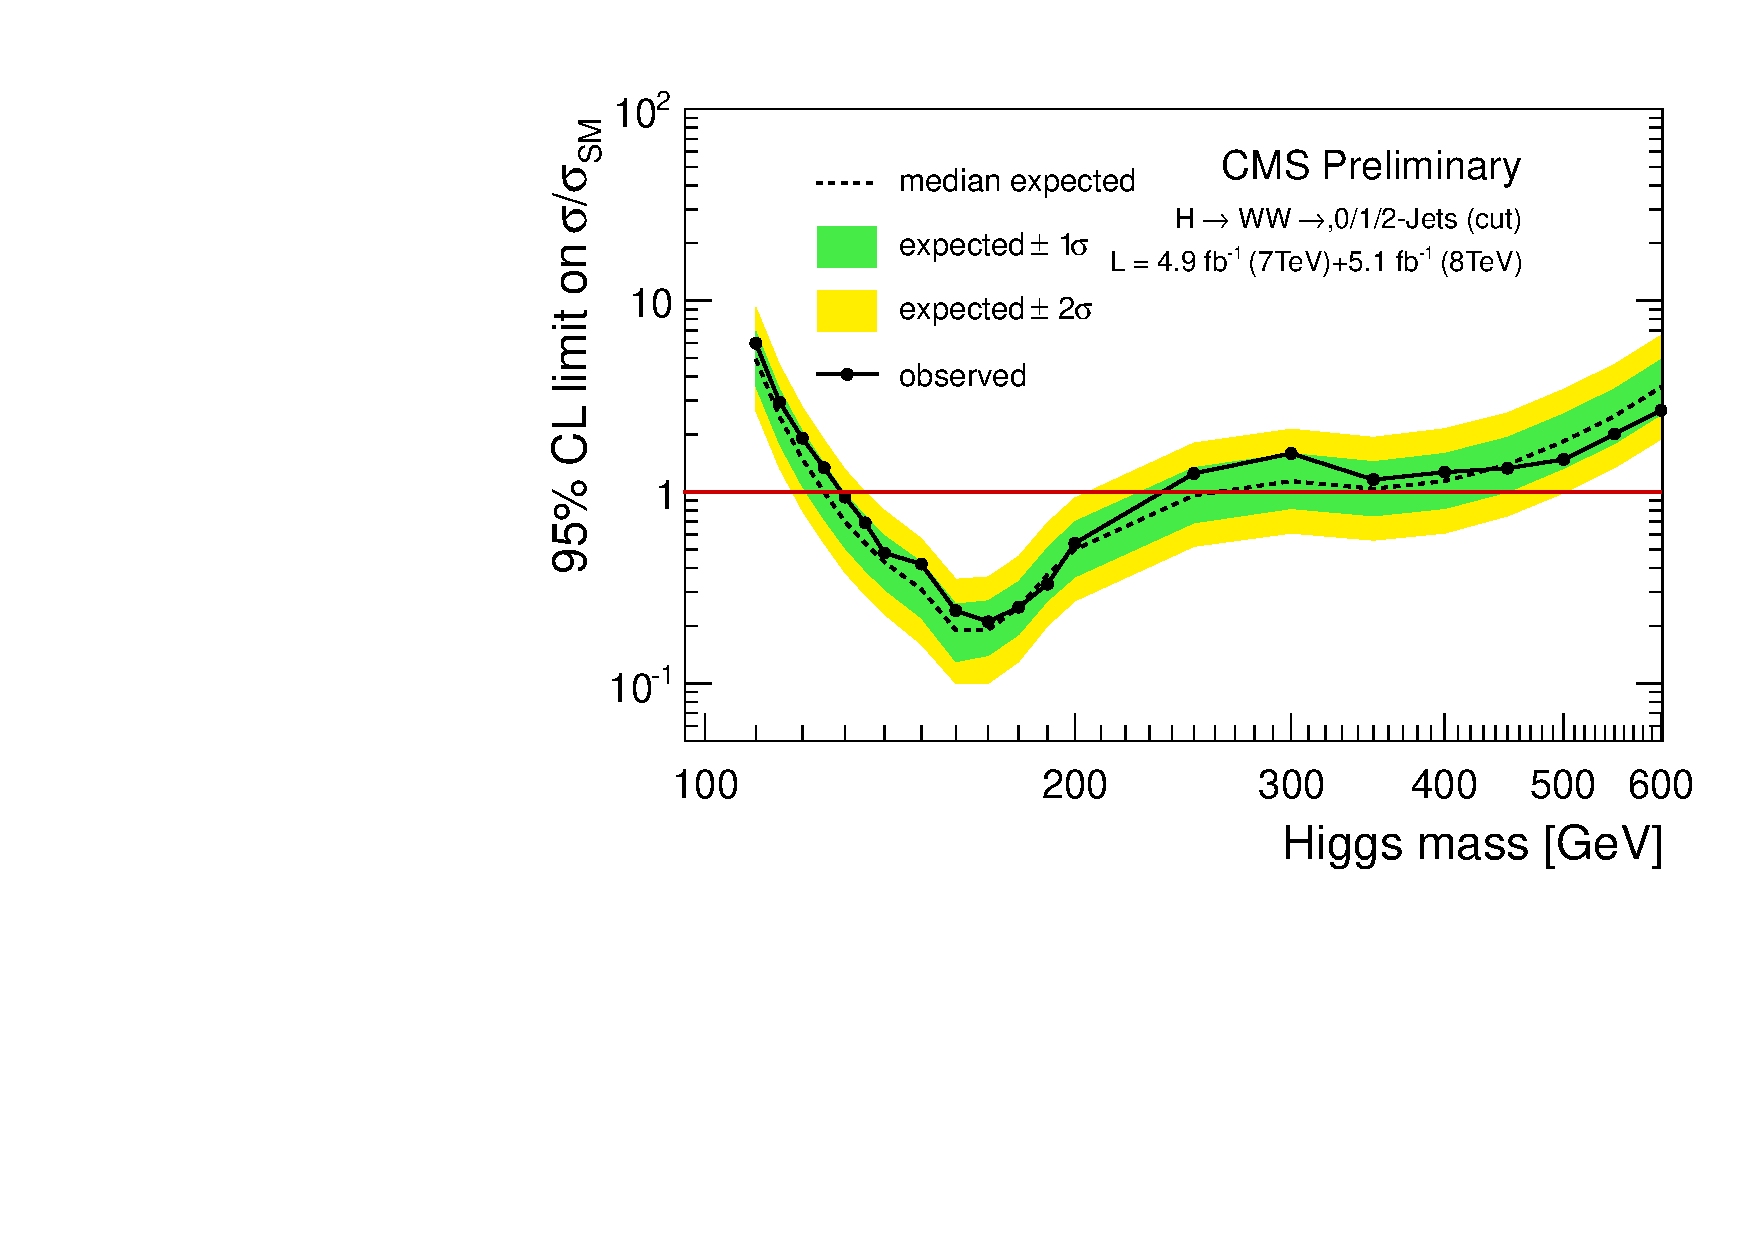
\includegraphics[width=.45\textwidth]{figures/limits_nj_cut_comb8tevof-CLs-asymptotic_log.pdf}} \\ 
\label{fig:uls_cut}
\caption{Expected and observed upper limits for SM Higgs using the
  {\bf cut-based} analysis using 7 TeV, 8 TeV and combined data. 
Note that for the 8 TeV cut-based results, we use only the 
{\bf OF final state in the 0/1-Jet bin}. }
\end{figure}


%%%%%%%%%%%%%%%%%%%%%%%%%%%%%%
\begin{table}[hbp!]
\begin{center}
\begin{tabular}{c c c c c}
\hline
\vspace{-3mm} && \\
 Higgs Mass & Observed  & Median expected & Expected range for 68\% & Expected range for 95\%   \\
\hline
\vspace{-3mm} && \\
110 & 5.98 & 4.94 & [3.56, 6.88] & [2.65, 9.22] \\
115 & 2.95 & 2.47 & [1.78, 3.44] & [1.33, 4.61] \\
120 & 1.91 & 1.49 & [1.07, 2.08] & [0.80, 2.78] \\
125 & 1.34 & 1.00 & [0.72, 1.40] & [0.54, 1.87] \\
130 & 0.94 & 0.70 & [0.51, 0.98] & [0.38, 1.31] \\
135 & 0.69 & 0.54 & [0.39, 0.75] & [0.29, 1.00] \\
140 & 0.48 & 0.43 & [0.31, 0.59] & [0.23, 0.80] \\
150 & 0.42 & 0.31 & [0.22, 0.43] & [0.16, 0.57] \\
160 & 0.24 & 0.19 & [0.13, 0.26] & [0.10, 0.35] \\
170 & 0.21 & 0.19 & [0.14, 0.27] & [0.10, 0.36] \\
180 & 0.25 & 0.25 & [0.18, 0.34] & [0.13, 0.46] \\
190 & 0.33 & 0.37 & [0.27, 0.51] & [0.20, 0.69] \\
200 & 0.54 & 0.50 & [0.36, 0.70] & [0.27, 0.93] \\
250 & 1.25 & 0.96 & [0.69, 1.34] & [0.52, 1.80] \\
300 & 1.59 & 1.14 & [0.82, 1.59] & [0.61, 2.13] \\
350 & 1.16 & 1.04 & [0.75, 1.44] & [0.56, 1.93] \\
400 & 1.27 & 1.14 & [0.82, 1.59] & [0.61, 2.14] \\
450 & 1.33 & 1.39 & [1.00, 1.93] & [0.75, 2.59] \\
500 & 1.48 & 1.84 & [1.33, 2.56] & [0.99, 3.44] \\
550 & 2.01 & 2.49 & [1.79, 3.46] & [1.34, 4.64] \\
600 & 2.67 & 3.53 & [2.54, 4.91] & [1.89, 6.58] \\
\hline
\end{tabular}
\caption{Expected and observed upper limits for SM Higgs using the
  {\bf cut-based} analysis, corresponding to $\intlumiSevenTeV$ at 7 TeV and $\intlumiEightTeV$ 8 TeV data. 
Note that for the 8 TeV data, only the {\bf OF final states in the 0/1-Jet bin} are included.}
\label{tab:cutbase_uls_7and8tevof}
\end{center}
\end{table}
%%%%%%%%%%%%%%%%%%%%%%%%%%%%%

%%%%%%%%%%%%%%%%%%%%%%%%%%%%%%%%%%%%%%%%%%%%%%%%%%%%%%%%%%%%
\begin{table}[hbp!]
\begin{center}
\begin{tabular}{c c c c c}
\hline
\vspace{-3mm} && \\
 Higgs Mass & Observed  & Median expected & Expected range for 68\% & Expected range for 95\%   \\
\hline
\vspace{-3mm} && \\
110 & 6.89 & 6.07 & [4.37, 8.45] & [3.26, 11.33] \\
115 & 3.16 & 2.90 & [2.09, 4.04] & [1.56, 5.41] \\
120 & 1.87 & 1.70 & [1.22, 2.37] & [0.91, 3.17] \\
125 & 1.37 & 1.16 & [0.84, 1.62] & [0.62, 2.17] \\
130 & 0.98 & 0.79 & [0.57, 1.10] & [0.42, 1.48] \\
135 & 0.75 & 0.62 & [0.45, 0.87] & [0.33, 1.16] \\
140 & 0.50 & 0.49 & [0.36, 0.69] & [0.26, 0.92] \\
150 & 0.44 & 0.38 & [0.27, 0.52] & [0.20, 0.70] \\
160 & 0.23 & 0.22 & [0.16, 0.31] & [0.12, 0.41] \\
170 & 0.22 & 0.23 & [0.16, 0.32] & [0.12, 0.42] \\
180 & 0.26 & 0.29 & [0.21, 0.41] & [0.16, 0.55] \\
190 & 0.34 & 0.43 & [0.31, 0.60] & [0.23, 0.80] \\
200 & 0.56 & 0.61 & [0.44, 0.85] & [0.33, 1.14] \\
250 & 1.05 & 1.16 & [0.84, 1.61] & [0.62, 2.16] \\
300 & 1.53 & 1.37 & [0.99, 1.91] & [0.74, 2.56] \\
350 & 1.38 & 1.28 & [0.92, 1.78] & [0.69, 2.39] \\
400 & 1.56 & 1.42 & [1.02, 1.97] & [0.76, 2.64] \\
450 & 1.84 & 1.76 & [1.27, 2.44] & [0.94, 3.28] \\
500 & 2.36 & 2.39 & [1.72, 3.32] & [1.28, 4.45] \\
550 & 3.48 & 3.30 & [2.38, 4.59] & [1.77, 6.16] \\
600 & 4.81 & 4.70 & [3.39, 6.54] & [2.52, 8.77] \\
\hline
\end{tabular}
\caption{Expected and observed upper limits for SM Higgs using the
  {\bf cut-based} analysis, corresponding to $\intlumiSevenTeV$ at 7 TeV. }
\label{tab:cutbase_uls_7tev}
\end{center}
%\end{table}
%%%%%%%%%%%%%%%%%%%%%%%%%%%%%%
%\begin{table}[hbp!]
\begin{center}
\begin{tabular}{c c c c c}
\hline
\vspace{-3mm} && \\
 Higgs Mass & Observed  & Median expected & Expected range for 68\% & Expected range for 95\%   \\
\vspace{-3mm} && \\
\hline
110 & 8.81 & 6.25 & [4.50, 8.70] & [3.35, 11.66] \\
115 & 4.76 & 3.29 & [2.37, 4.58] & [1.77, 6.14] \\
120 & 3.14 & 1.98 & [1.43, 2.75] & [1.06, 3.69] \\
125 & 1.95 & 1.29 & [0.93, 1.79] & [0.69, 2.40] \\
130 & 1.39 & 0.93 & [0.67, 1.29] & [0.50, 1.73] \\
135 & 0.99 & 0.69 & [0.50, 0.96] & [0.37, 1.29] \\
140 & 0.76 & 0.56 & [0.40, 0.78] & [0.30, 1.05] \\
145 & 0.70 & 0.48 & [0.35, 0.67] & [0.26, 0.90] \\
150 & 0.56 & 0.38 & [0.27, 0.53] & [0.20, 0.71] \\
160 & 0.37 & 0.23 & [0.16, 0.31] & [0.12, 0.42] \\
170 & 0.34 & 0.25 & [0.18, 0.34] & [0.13, 0.46] \\
180 & 0.43 & 0.33 & [0.24, 0.46] & [0.18, 0.62] \\
190 & 0.69 & 0.52 & [0.37, 0.72] & [0.28, 0.97] \\
200 & 0.95 & 0.65 & [0.47, 0.91] & [0.35, 1.21] \\
250 & 2.21 & 1.24 & [0.90, 1.73] & [0.67, 2.32] \\
300 & 2.31 & 1.46 & [1.05, 2.03] & [0.78, 2.73] \\
350 & 1.47 & 1.29 & [0.93, 1.80] & [0.69, 2.41] \\
400 & 1.57 & 1.46 & [1.05, 2.03] & [0.78, 2.72] \\
450 & 1.64 & 1.83 & [1.32, 2.55] & [0.98, 3.41] \\
500 & 1.79 & 2.45 & [1.76, 3.41] & [1.31, 4.57] \\
550 & 2.33 & 3.30 & [2.38, 4.59] & [1.77, 6.16] \\
600 & 3.15 & 4.74 & [3.42, 6.60] & [2.55, 8.85] \\
\hline
\end{tabular}
\caption{Expected and observed upper limits for SM Higgs using the
  {\bf cut-based} analysis with \intlumiEightTeV\ of data at 8 TeV. 
Note that we include only the {\bf OF final states in the 0/1-Jet bins}.}
\label{tab:cutbase_uls_8tev_of}
\end{center}
\end{table}
\clearpage

\subsection{Detailed Results at 8 TeV}

%%%%%%%%%%%%%%%%%%%%%%%%%%%%%%
\begin{figure}[!hbtp]
\centering
\subfigure[SM Higgs (cut-based) 8 TeV 0-Jet OF ]{
\centering
\label{subfig:sm_cut_8tev_0jof}
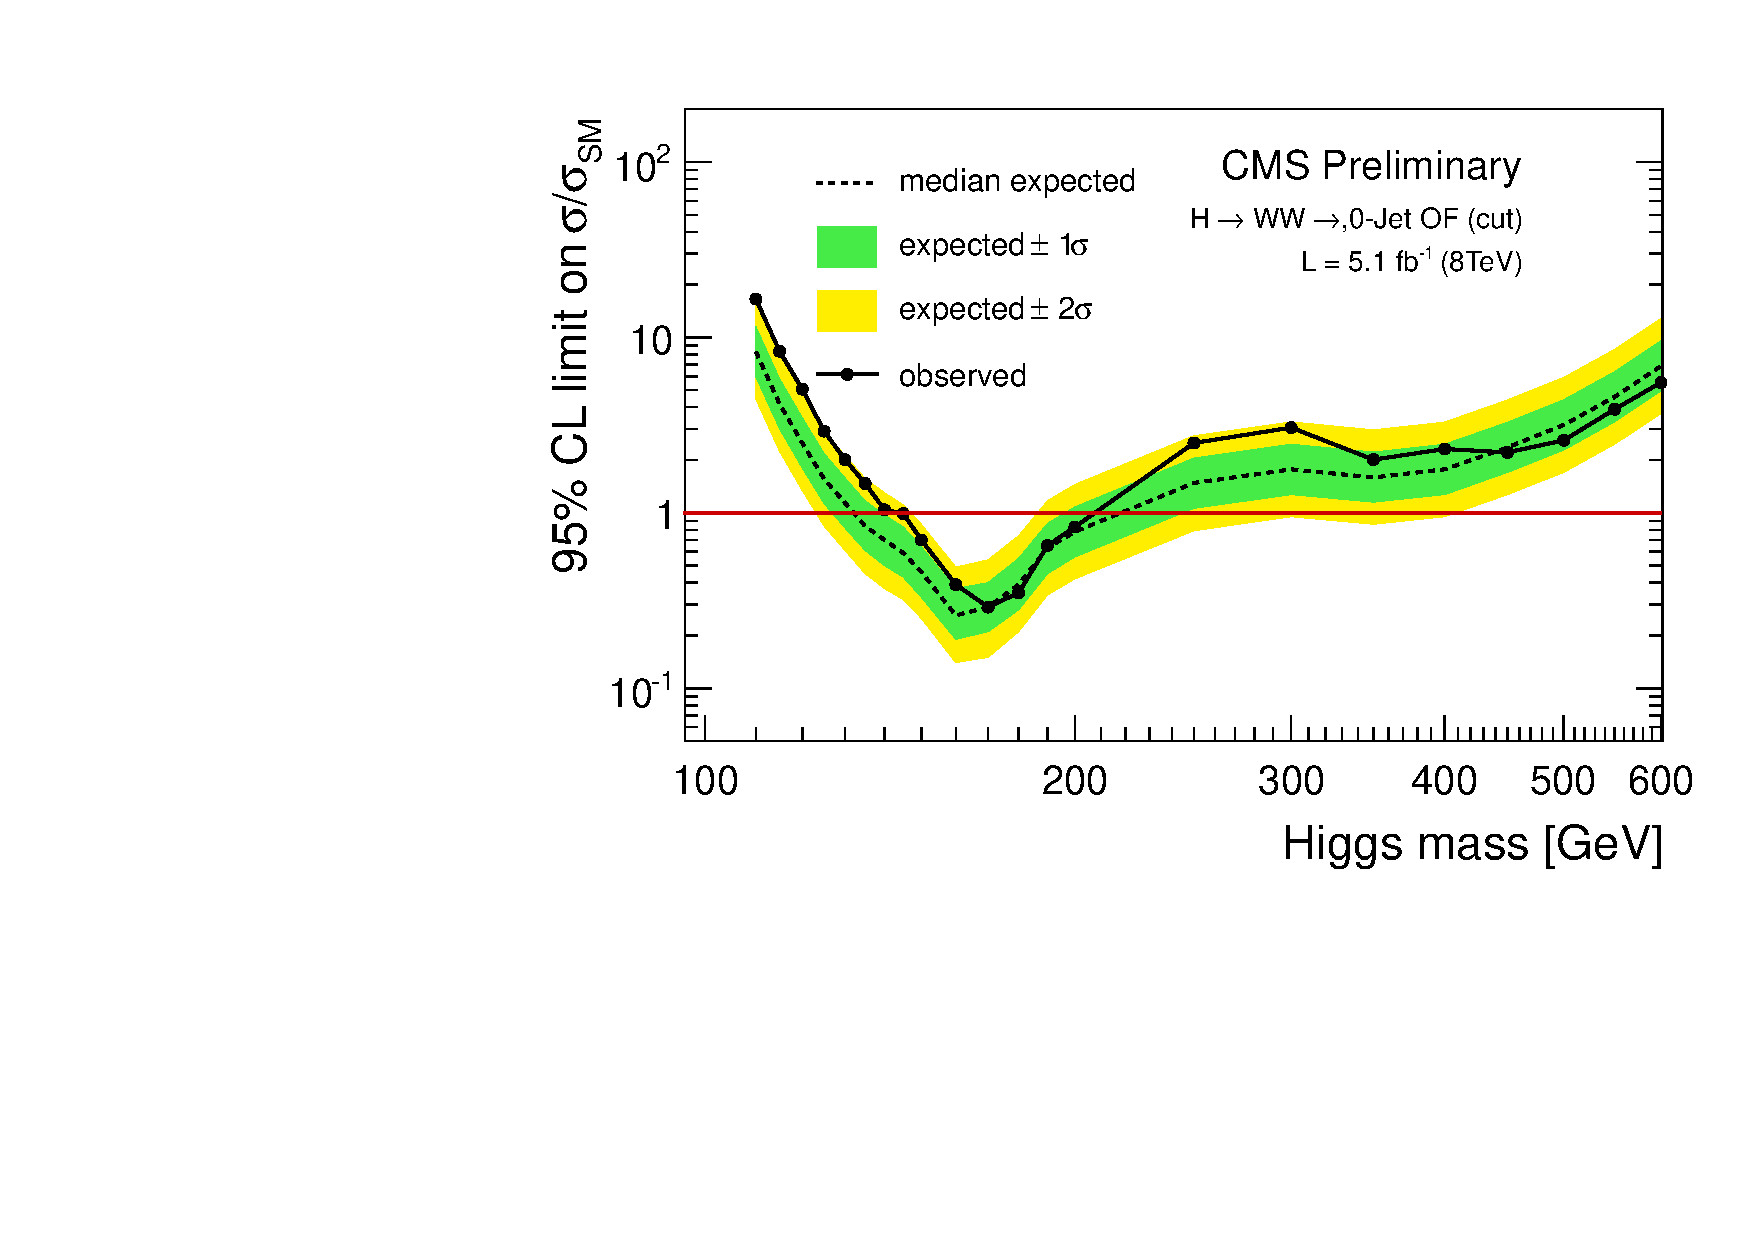
\includegraphics[width=.45\textwidth]{figures/limits_0jof_cut_8TeV-CLs-asymptotic_log.pdf}}
\subfigure[SM Higgs (cut-based) 8 TeV 0-Jet SF ]{
\centering
\label{subfig:sm_cut_8tev_0jof}
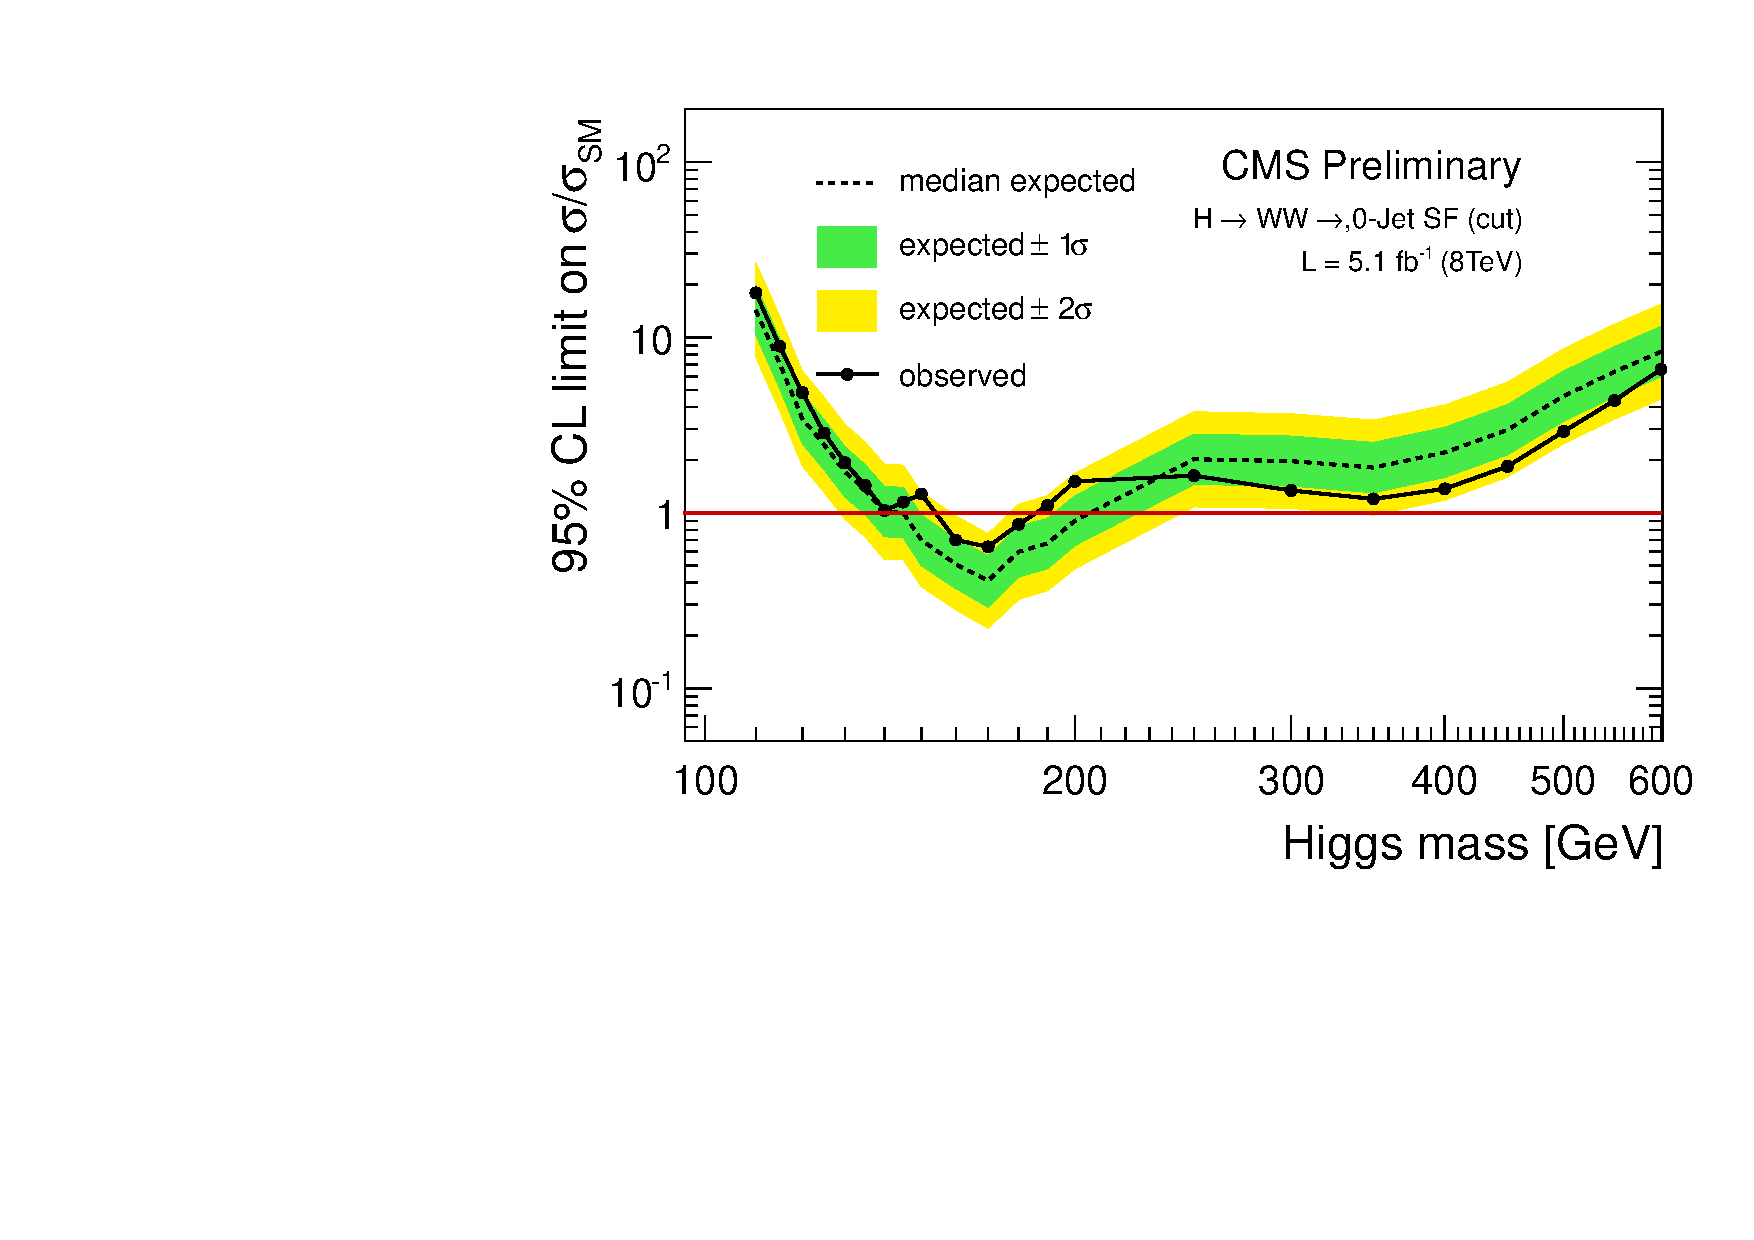
\includegraphics[width=.45\textwidth]{figures/limits_0jsf_cut_8TeV-CLs-asymptotic_log.pdf}} \\
\subfigure[SM Higgs (cut-based) 8 TeV 1-Jet OF ]{
\centering
\label{subfig:sm_cut_8tev_0jof}
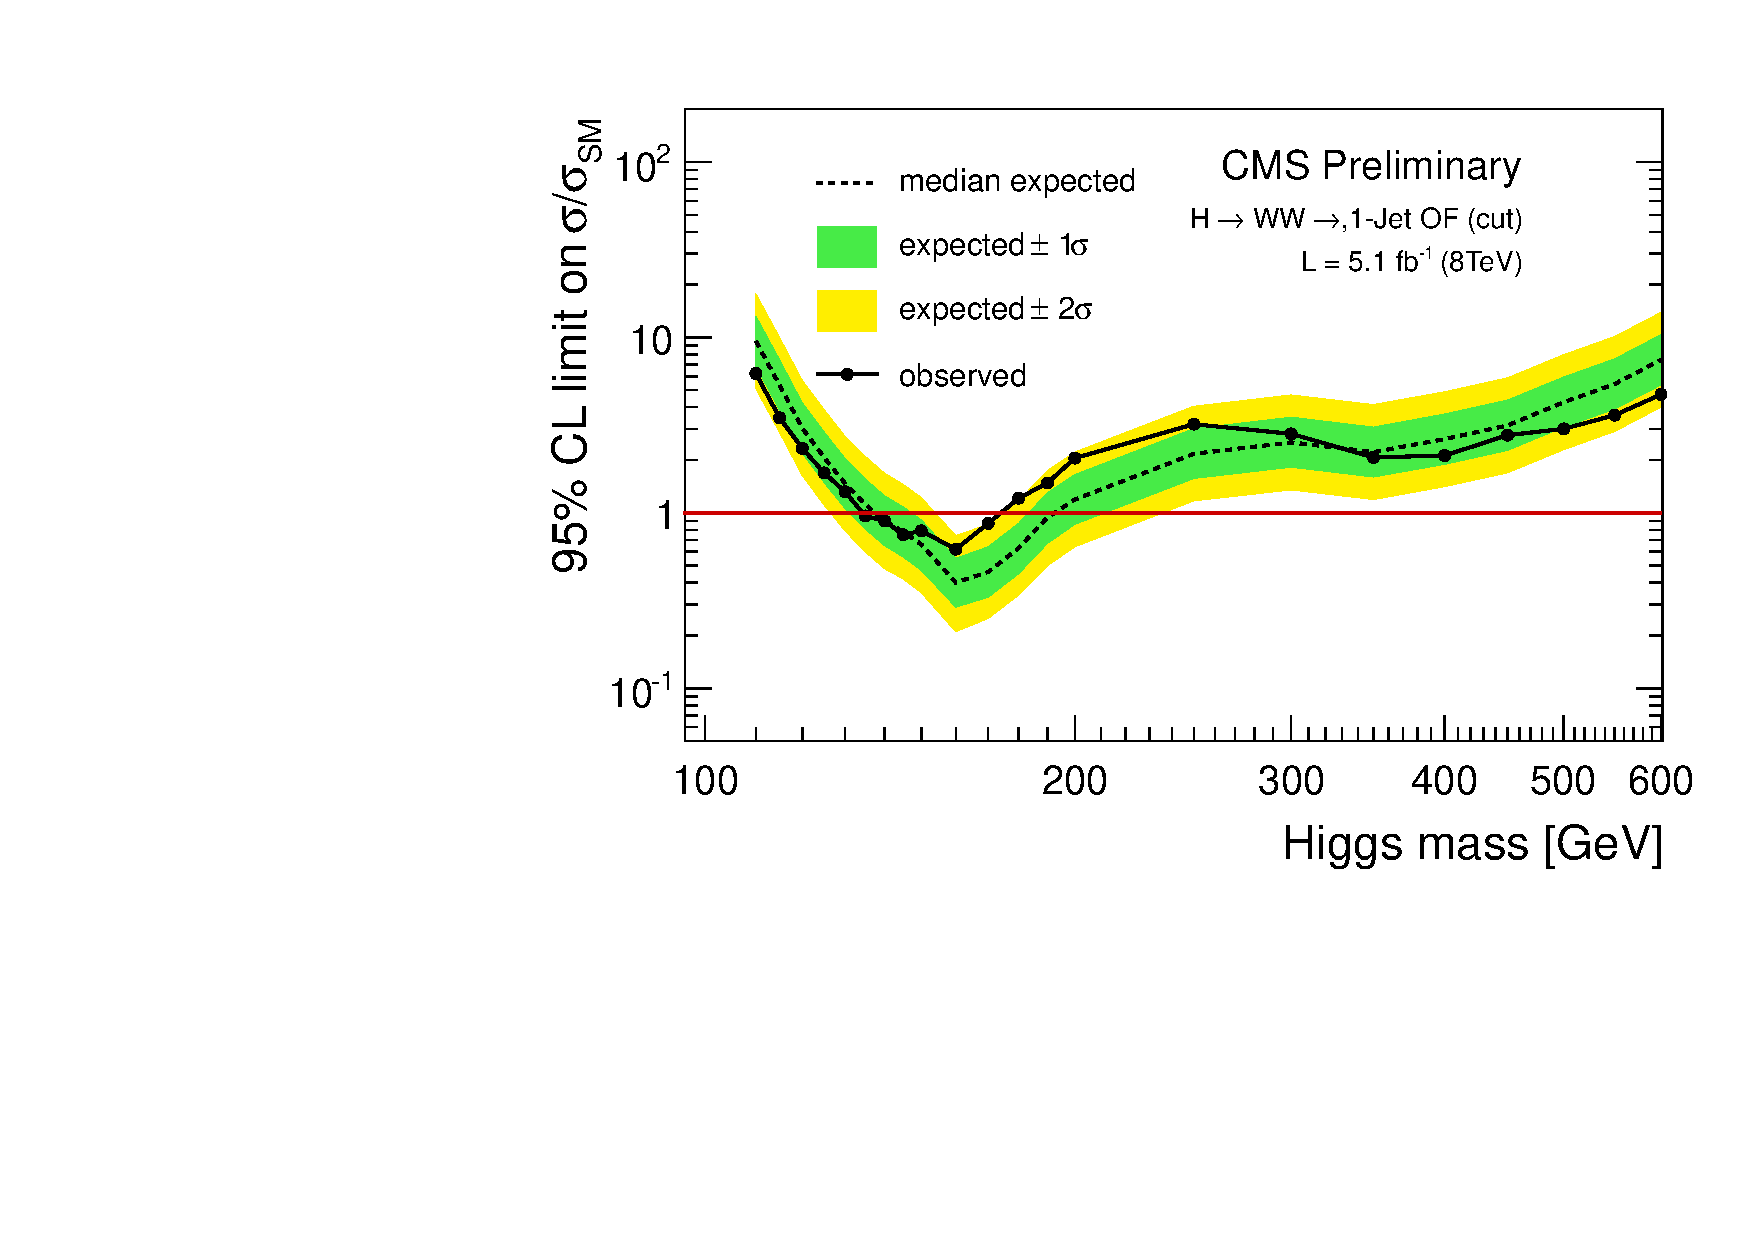
\includegraphics[width=.45\textwidth]{figures/limits_1jof_cut_8TeV-CLs-asymptotic_log.pdf}}
\subfigure[SM Higgs (cut-based) 8 TeV 1-Jet SF ]{
\centering
\label{subfig:sm_cut_8tev_0jof}
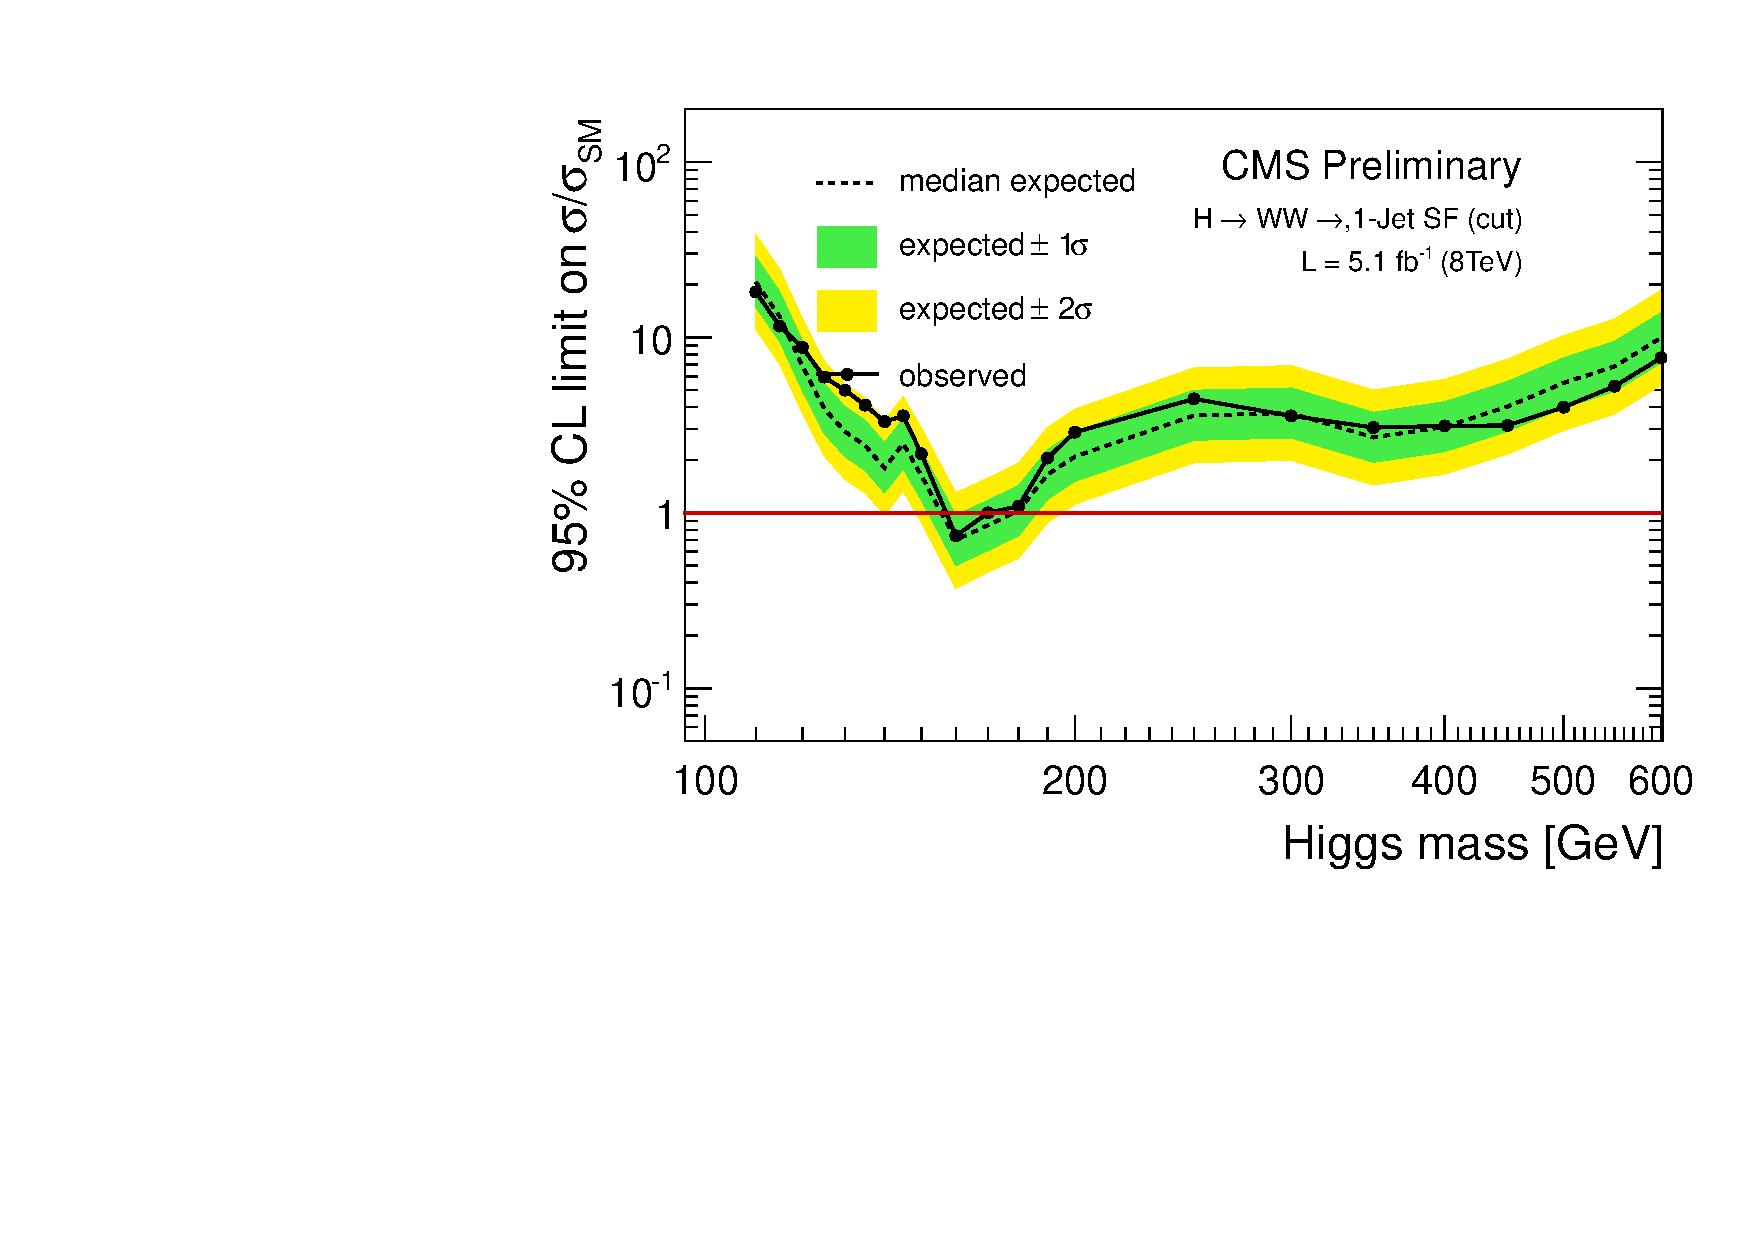
\includegraphics[width=.45\textwidth]{figures/limits_1jsf_cut_8TeV-CLs-asymptotic_log.pdf}} \\
\subfigure[SM Higgs (cut-based) 8 TeV 2-Jet OF ]{
\centering
\label{subfig:sm_cut_8tev_0jof}
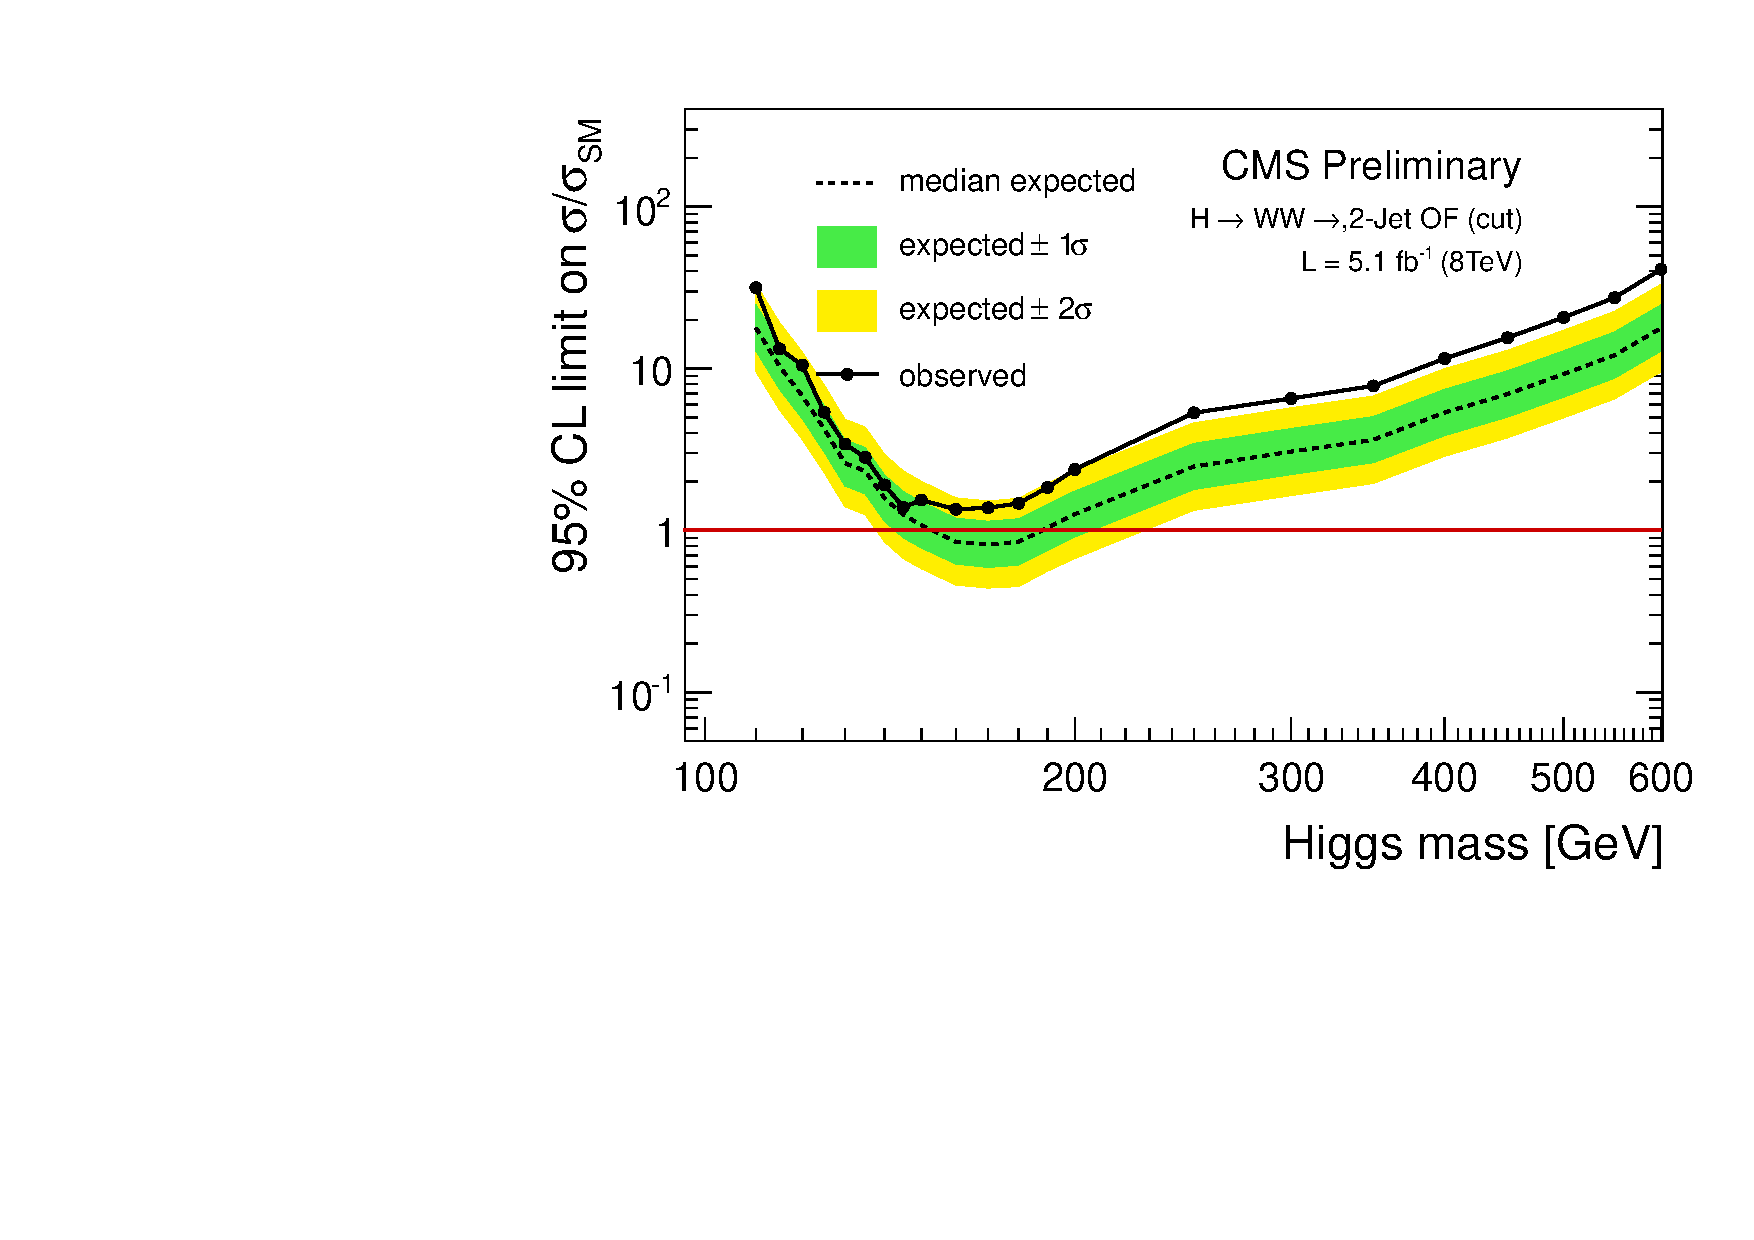
\includegraphics[width=.45\textwidth]{figures/limits_2jof_cut_8TeV-CLs-asymptotic_log.pdf}}
\subfigure[SM Higgs (cut-based) 8 TeV 2-Jet SF ]{
\centering
\label{subfig:sm_cut_8tev_0jof}
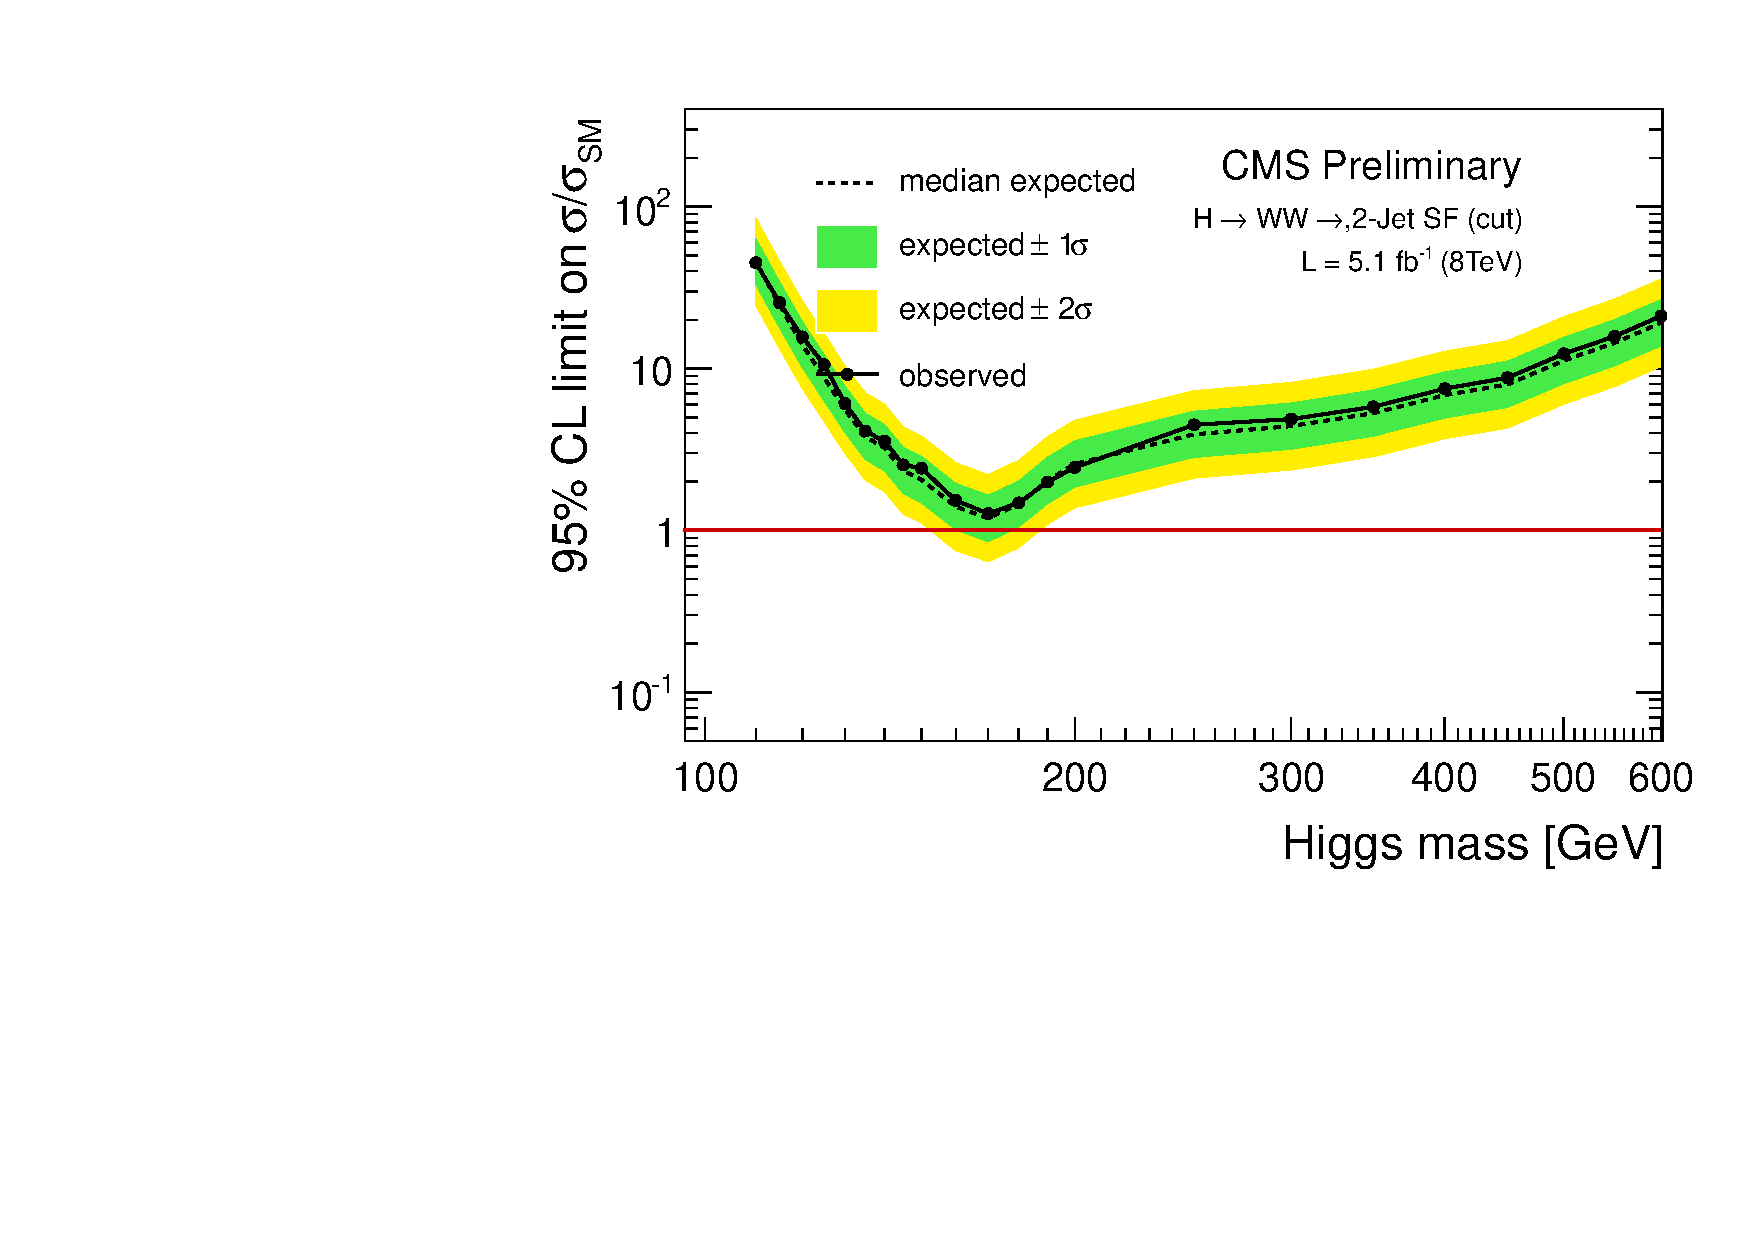
\includegraphics[width=.45\textwidth]{figures/limits_2jsf_cut_8TeV-CLs-asymptotic_log.pdf}} \\
\label{fig:uls_cut_8tev}
\caption{Expected and observed upper limits for SM Higgs using the
  {\bf cut-based} analysis using {\bf 8 TeV data}.}
\end{figure}
%%%%%%%%%%%%%%%%%%%%%%%%%%%%%%%%%%%%%%%%%%%%%%%%%%%%%%%%%%%%
%%%%%%%%%%%%%%%%%%%%%%%%%%%%%%
\begin{table}[hbp!]
\begin{center}
\begin{tabular}{c c c c c}
\hline
\vspace{-3mm} && \\
 Higgs Mass & Observed  & Median expected & Expected range for 68\% & Expected range for 95\%   \\
\vspace{-3mm} && \\
\hline
\multicolumn{5}{c}{0-Jet OF} \\
\hline
110 & 16.54 & 8.28 & [5.96, 11.52] & [4.44, 15.44] \\
115 & 8.33 & 4.17 & [3.01, 5.81] & [2.24, 7.79] \\
120 & 5.07 & 2.50 & [1.80, 3.48] & [1.34, 4.67] \\
125 & 2.92 & 1.56 & [1.13, 2.18] & [0.84, 2.92] \\
130 & 2.01 & 1.14 & [0.82, 1.58] & [0.61, 2.12] \\
135 & 1.47 & 0.84 & [0.61, 1.17] & [0.45, 1.57] \\
140 & 1.04 & 0.70 & [0.50, 0.97] & [0.37, 1.30] \\
145 & 0.99 & 0.59 & [0.43, 0.83] & [0.32, 1.11] \\
150 & 0.70 & 0.46 & [0.33, 0.64] & [0.25, 0.86] \\
160 & 0.39 & 0.26 & [0.19, 0.37] & [0.14, 0.49] \\
170 & 0.29 & 0.29 & [0.21, 0.40] & [0.15, 0.54] \\
180 & 0.35 & 0.39 & [0.28, 0.55] & [0.21, 0.74] \\
190 & 0.65 & 0.63 & [0.45, 0.87] & [0.34, 1.17] \\
200 & 0.83 & 0.78 & [0.56, 1.08] & [0.42, 1.45] \\
250 & 2.50 & 1.48 & [1.06, 2.05] & [0.79, 2.75] \\
300 & 3.06 & 1.77 & [1.27, 2.46] & [0.95, 3.30] \\
350 & 2.01 & 1.59 & [1.15, 2.22] & [0.86, 2.97] \\
400 & 2.31 & 1.77 & [1.27, 2.46] & [0.95, 3.29] \\
450 & 2.21 & 2.36 & [1.70, 3.28] & [1.27, 4.40] \\
500 & 2.59 & 3.17 & [2.28, 4.41] & [1.70, 5.91] \\
550 & 3.89 & 4.58 & [3.30, 6.37] & [2.46, 8.54] \\
600 & 5.53 & 6.86 & [4.95, 9.55] & [3.68, 12.81] \\
110 & 17.93 & 14.28 & [10.29, 19.87] & [7.66, 26.64] \\
\hline
\multicolumn{5}{c}{0-Jet SF} \\
\hline
115 & 8.92 & 7.11 & [5.12, 9.89] & [3.82, 13.26] \\
120 & 4.85 & 3.45 & [2.48, 4.80] & [1.85, 6.43] \\
125 & 2.85 & 2.45 & [1.76, 3.40] & [1.31, 4.56] \\
130 & 1.93 & 1.71 & [1.23, 2.38] & [0.92, 3.19] \\
135 & 1.43 & 1.35 & [0.98, 1.88] & [0.73, 2.53] \\
140 & 1.03 & 1.01 & [0.73, 1.41] & [0.54, 1.89] \\
145 & 1.15 & 1.00 & [0.72, 1.40] & [0.54, 1.87] \\
150 & 1.28 & 0.70 & [0.50, 0.97] & [0.38, 1.31] \\
160 & 0.70 & 0.51 & [0.37, 0.71] & [0.28, 0.96] \\
170 & 0.64 & 0.41 & [0.29, 0.57] & [0.22, 0.76] \\
180 & 0.86 & 0.60 & [0.43, 0.84] & [0.32, 1.12] \\
190 & 1.10 & 0.67 & [0.48, 0.93] & [0.36, 1.25] \\
200 & 1.51 & 0.90 & [0.65, 1.25] & [0.48, 1.68] \\
250 & 1.63 & 2.02 & [1.45, 2.81] & [1.08, 3.77] \\
300 & 1.34 & 1.97 & [1.42, 2.74] & [1.06, 3.67] \\
350 & 1.20 & 1.81 & [1.30, 2.52] & [0.97, 3.38] \\
400 & 1.37 & 2.21 & [1.59, 3.07] & [1.18, 4.12] \\
450 & 1.84 & 2.97 & [2.14, 4.14] & [1.60, 5.55] \\
500 & 2.91 & 4.63 & [3.33, 6.44] & [2.48, 8.63] \\
550 & 4.37 & 6.37 & [4.59, 8.87] & [3.42, 11.89] \\
600 & 6.58 & 8.29 & [5.97, 11.54] & [4.45, 15.47] \\

\hline
\end{tabular}
\caption{Expected and observed upper limits for SM Higgs using the
  {\bf cut-based} analysis with \intlumiEightTeV\ of data in the {\bf 0-Jet} final state.}
\label{tab:cutbase_uls_0j}
\end{center}
\end{table}
%%%%%%%%%%%%%%%%%%%%%%%%%%%%%%

%%%%%%%%%%%%%%%%%%%%%%%%%%%%%%%%%%%%%%%%%%%%%%%%%%%%%%%%%%%%
%%%%%%%%%%%%%%%%%%%%%%%%%%%%%%
\begin{table}[hbp!]
\begin{center}
\begin{tabular}{c c c c c}
\hline
\vspace{-3mm} && \\
 Higgs Mass & Observed  & Median expected & Expected range for 68\% & Expected range for 95\%   \\
\vspace{-3mm} && \\
\hline
\multicolumn{5}{c}{1-Jet OF} \\
\hline
110 & 6.22 & 9.50 & [6.85, 13.22] & [5.10, 17.73] \\
115 & 3.48 & 5.34 & [3.85, 7.44] & [2.87, 9.97] \\
120 & 2.33 & 3.04 & [2.19, 4.23] & [1.63, 5.68] \\
125 & 1.69 & 2.07 & [1.49, 2.89] & [1.11, 3.87] \\
130 & 1.32 & 1.47 & [1.06, 2.04] & [0.79, 2.73] \\
135 & 0.96 & 1.12 & [0.81, 1.56] & [0.60, 2.10] \\
140 & 0.90 & 0.90 & [0.65, 1.25] & [0.48, 1.68] \\
145 & 0.75 & 0.78 & [0.56, 1.08] & [0.42, 1.45] \\
150 & 0.79 & 0.66 & [0.47, 0.91] & [0.35, 1.22] \\
160 & 0.62 & 0.40 & [0.29, 0.55] & [0.21, 0.74] \\
170 & 0.87 & 0.46 & [0.33, 0.64] & [0.25, 0.86] \\
180 & 1.21 & 0.63 & [0.45, 0.87] & [0.34, 1.17] \\
190 & 1.48 & 0.94 & [0.67, 1.30] & [0.50, 1.74] \\
200 & 2.05 & 1.19 & [0.86, 1.65] & [0.64, 2.22] \\
250 & 3.20 & 2.17 & [1.57, 3.02] & [1.17, 4.05] \\
300 & 2.82 & 2.52 & [1.82, 3.51] & [1.35, 4.70] \\
350 & 2.07 & 2.22 & [1.60, 3.08] & [1.19, 4.14] \\
400 & 2.12 & 2.63 & [1.89, 3.66] & [1.41, 4.90] \\
450 & 2.77 & 3.15 & [2.27, 4.39] & [1.69, 5.88] \\
500 & 3.01 & 4.27 & [3.08, 5.94] & [2.29, 7.97] \\
550 & 3.60 & 5.42 & [3.90, 7.54] & [2.91, 10.11] \\
600 & 4.73 & 7.45 & [5.36, 10.36] & [4.00, 13.89] \\
\hline
\multicolumn{5}{c}{1-Jet SF} \\
\hline
110 & 18.15 & 20.66 & [14.88, 28.74] & [11.09, 38.53] \\
115 & 11.60 & 13.18 & [9.49, 18.34] & [7.07, 24.58] \\
120 & 8.76 & 6.90 & [4.97, 9.60] & [3.70, 12.87] \\
125 & 5.94 & 3.93 & [2.83, 5.47] & [2.11, 7.33] \\
130 & 5.00 & 2.90 & [2.09, 4.03] & [1.55, 5.40] \\
135 & 4.11 & 2.42 & [1.74, 3.37] & [1.30, 4.52] \\
140 & 3.31 & 1.80 & [1.30, 2.51] & [0.97, 3.36] \\
145 & 3.57 & 2.48 & [1.78, 3.44] & [1.33, 4.62] \\
150 & 2.17 & 1.63 & [1.18, 2.27] & [0.88, 3.05] \\
160 & 0.74 & 0.70 & [0.50, 0.97] & [0.37, 1.30] \\
170 & 1.00 & 0.85 & [0.61, 1.18] & [0.46, 1.58] \\
180 & 1.09 & 1.03 & [0.74, 1.43] & [0.55, 1.92] \\
190 & 2.05 & 1.65 & [1.19, 2.29] & [0.88, 3.07] \\
200 & 2.88 & 2.09 & [1.51, 2.91] & [1.12, 3.90] \\
250 & 4.46 & 3.59 & [2.59, 5.00] & [1.93, 6.70] \\
300 & 3.57 & 3.70 & [2.67, 5.15] & [1.99, 6.90] \\
350 & 3.06 & 2.69 & [1.94, 3.74] & [1.44, 5.01] \\
% 350 & 3.06 & 35.57 & [25.62, 49.49] & [19.09, 66.34] \\ rMax = 50 in the expected
400 & 3.13 & 3.09 & [2.23, 4.30] & [1.66, 5.77] \\
450 & 3.15 & 4.03 & [2.91, 5.61] & [2.16, 7.52] \\
500 & 4.00 & 5.50 & [3.96, 7.65] & [2.95, 10.25] \\
550 & 5.27 & 6.83 & [4.92, 9.50] & [3.66, 12.73] \\
600 & 7.64 & 9.95 & [7.16, 13.84] & [5.34, 18.55] \\
\hline
\end{tabular}
\caption{Expected and observed upper limits for SM Higgs using the
  {\bf cut-based} analysis with \intlumiEightTeV\ of data in the {\bf 1-Jet} final state.}
\label{tab:cutbase_uls_1j}
\end{center}
\end{table}
%%%%%%%%%%%%%%%%%%%%%%%%%%%%%%

%%%%%%%%%%%%%%%%%%%%%%%%%%%%%%%%%%%%%%%%%%%%%%%%%%%%%%%%%%%%
%%%%%%%%%%%%%%%%%%%%%%%%%%%%%%
\begin{table}[hbp!]
\begin{center}
\begin{tabular}{c c c c c}
\hline
\vspace{-3mm} && \\
 Higgs Mass & Observed  & Median expected & Expected range for 68\% & Expected range for 95\%   \\
\vspace{-3mm} && \\
\hline
\multicolumn{5}{c}{2-Jet OF} \\
\hline
110 & 31.60 & 17.83 & [12.85, 24.81] & [9.57, 33.27] \\
115 & 13.23 & 10.32 & [7.44, 14.36] & [5.54, 19.25] \\
120 & 10.49 & 6.78 & [4.89, 9.44] & [3.64, 12.65] \\
125 & 5.37 & 4.25 & [3.06, 5.92] & [2.28, 7.93] \\
130 & 3.42 & 2.60 & [1.88, 3.62] & [1.40, 4.86] \\
135 & 2.83 & 2.33 & [1.68, 3.25] & [1.25, 4.35] \\
140 & 1.91 & 1.58 & [1.14, 2.20] & [0.85, 2.95] \\
145 & 1.39 & 1.25 & [0.90, 1.74] & [0.67, 2.33] \\
150 & 1.54 & 1.08 & [0.78, 1.50] & [0.58, 2.01] \\
160 & 1.35 & 0.85 & [0.62, 1.19] & [0.46, 1.59] \\
170 & 1.38 & 0.82 & [0.59, 1.14] & [0.44, 1.52] \\
180 & 1.47 & 0.85 & [0.61, 1.18] & [0.45, 1.58] \\
190 & 1.84 & 1.04 & [0.75, 1.45] & [0.56, 1.95] \\
200 & 2.38 & 1.26 & [0.91, 1.75] & [0.67, 2.35] \\
250 & 5.33 & 2.48 & [1.79, 3.45] & [1.33, 4.62] \\
300 & 6.53 & 3.07 & [2.21, 4.26] & [1.64, 5.72] \\
350 & 7.81 & 3.63 & [2.62, 5.05] & [1.95, 6.77] \\
400 & 11.52 & 5.35 & [3.85, 7.44] & [2.87, 9.98] \\
450 & 15.50 & 6.95 & [5.01, 9.68] & [3.73, 12.97] \\
500 & 20.69 & 9.25 & [6.66, 12.87] & [4.96, 17.25] \\
550 & 27.39 & 12.09 & [8.71, 16.82] & [6.49, 22.55] \\
600 & 40.99 & 17.78 & [12.81, 24.73] & [9.54, 33.16] \\
\hline
\multicolumn{5}{c}{2-Jet SF} \\
\hline
110 & 45.07 & 45.69 & [32.92, 63.58] & [24.52, 85.23] \\
115 & 25.51 & 24.68 & [17.78, 34.34] & [13.24, 46.04] \\
120 & 15.68 & 14.05 & [10.12, 19.55] & [7.54, 26.21] \\
125 & 10.57 & 8.78 & [6.32, 12.21] & [4.71, 16.37] \\
130 & 6.08 & 5.58 & [4.02, 7.76] & [2.99, 10.40] \\
135 & 4.11 & 3.81 & [2.75, 5.31] & [2.05, 7.11] \\
140 & 3.55 & 3.23 & [2.33, 4.50] & [1.73, 6.03] \\
145 & 2.54 & 2.34 & [1.69, 3.26] & [1.26, 4.36] \\
150 & 2.42 & 2.06 & [1.48, 2.87] & [1.11, 3.84] \\
160 & 1.53 & 1.40 & [1.01, 1.95] & [0.75, 2.62] \\
170 & 1.27 & 1.19 & [0.85, 1.65] & [0.64, 2.21] \\
180 & 1.48 & 1.45 & [1.05, 2.02] & [0.78, 2.71] \\
190 & 1.99 & 2.03 & [1.46, 2.83] & [1.09, 3.79] \\

250 & 4.49 & 3.92 & [2.82, 5.45] & [2.10, 7.30] \\
300 & 4.87 & 4.41 & [3.17, 6.13] & [2.36, 8.22] \\
350 & 5.80 & 5.30 & [3.82, 7.38] & [2.85, 9.90] \\
400 & 7.51 & 6.85 & [4.94, 9.53] & [3.68, 12.78] \\
450 & 8.77 & 7.98 & [5.75, 11.10] & [4.28, 14.88] \\
500 & 12.34 & 11.19 & [8.06, 15.57] & [6.01, 20.88] \\
550 & 15.80 & 14.41 & [10.38, 20.05] & [7.73, 26.87] \\
600 & 21.09 & 19.16 & [13.80, 26.66] & [10.28, 35.73] \\
\hline
\end{tabular}
\caption{Expected and observed upper limits for SM Higgs using the
  {\bf cut-based} analysis with \intlumiEightTeV\ of data in the {\bf 2-Jet} final state.}
\label{tab:cutbase_uls_2j}
\end{center}
\end{table}
%%%%%%%%%%%%%%%%%%%%%%%%%%%%%%

